% main.tex
\documentclass{book/custombook}

\unitname{Systems Programming}
\unitcode{CAB403}
\unitcoordinator{Timothy Chappell}
\author{Dinal Atapattu}

\begin{document}
\maketitle

\section{Introduction}
\lipsum[1-5]

\begin{figure}[H]
    \centering
    \begin{subfigure}{0.5\textwidth}
        \centering
        \begin{tabular}{ccc}
            Process & Burst Time & Arrival Time\\
            \toprule
            P1 & 24 & 0\\
            P2 & 3  & 1\\
            P3 & 3  & 2\\
            \bottomrule
        \end{tabular}
        \caption{Process Table}
    \end{subfigure}%
    \begin{subfigure}{0.5\textwidth}
        \centering
        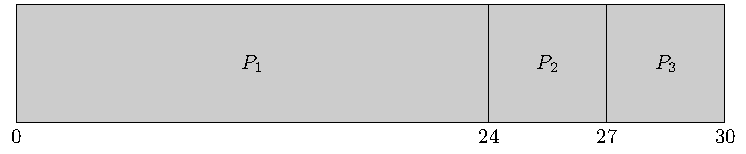
\includegraphics[width=\linewidth]{figures/fifo_gantt_1.pdf}
        \caption{FIFO Gantt Chart}
    \end{subfigure}
    Waiting time for $P_1$ is 0, $P_2$ is 24, $P_3$ is 27. Average waiting time is 17.
    \caption{Process Table and FIFO Gantt Chart with waiting times}
\end{figure}

\end{document}
